% Document uses 12 pt font
% 1 in margins
% Contains a relative path for images

\documentclass [10pt]{article}

% page geometry 
\usepackage[margin=1in]{geometry}


% ----------  PACKAGES START ------------ %
% Math Packages
\usepackage{amsmath}
\usepackage{mathtools}

% Table cell color package and highlighting
\usepackage[table]{xcolor}
\usepackage{color,soul}

% VIC title package
\usepackage{cabin}
\usepackage[T1]{fontenc}

% default font package
%\usepackage{times}
\usepackage{helvet}
%\renewcommand{\familydefault}{\sfdefault}

% ---------- End Font Packages -------------- %

\usepackage{listings}


\definecolor{dkgreen}{rgb}{0,0.6,0}
\definecolor{gray}{rgb}{0.5,0.5,0.5}
\definecolor{mauve}{rgb}{0.58,0,0.82}

\lstset{frame=tb,
  language=C++,
  aboveskip=3mm,
  belowskip=3mm,
  showstringspaces=false,
  columns=flexible,
  basicstyle={\small\ttfamily},
  numbers=none,
  numberstyle=\tiny\color{gray},
  keywordstyle=\color{blue},
  commentstyle=\color{dkgreen},
  stringstyle=\color{mauve},
  breaklines=true,
  breakatwhitespace=true,
  tabsize=3
}

% Title Packages
\usepackage{titlesec}
\usepackage{titletoc}

% Image Package
\usepackage{graphicx}

% Table Packages
\usepackage{longtable}
\usepackage{multirow}
\usepackage{multicol}
\usepackage{multirow}
\usepackage{array}
\renewcommand{\arraystretch}{1.4}% Spread rows out evenly in table
\setlength{\LTpre}{0.5pt} % Reduces white space around tables (top)
%\setlength{\LTpost}{0pt} % Reduces white space around tables (bottom)

% Color Packages
\usepackage{color}   
\definecolor{sectionC}{rgb}{0.016,0.227,.365}
\definecolor{subsectionC}{rgb}{.87,0.87,.87}
\definecolor{subsubsectionC}{rgb}{.94,.93,.90}
\definecolor{tableCell}{rgb}{.96,.95,.90}


% List package
\usepackage{enumitem}
\setenumerate{itemsep=0pt, itemindent=0in,leftmargin=0.5in}


% Paragraph parameter

\setlength{\parindent}{0pt}


% ------------- Creates a linked Table of Contents  Start --------------- %
\usepackage{hyperref}
\hypersetup{
colorlinks=true, %set true if you want colored links
linktoc=all,     %set to all if you want both sections and subsections linked
linkcolor=black,}  %choose some color if you want links to stand out

% ------------- Creates a click-able Table of Contents  End--------------- %

% ---------- PACKAGES END ------------ %








% -------- SECTION AND SUBSECTION FORMATING START -------- % 
% starts the 
%\setcounter{section}{1}


\titleformat{\section} % Section
{\normalfont \fontsize{14}{14} \bfseries}{}{0em}{\colorsection}

% Makes a background color
\newcommand{\colorsection}[1]{%
  \colorbox{sectionC}{\parbox{\dimexpr\textwidth-1\fboxsep}{\color{white}\Large\thesection\ \hspace{1mm} #1}}}

% Makes a background color
\titleformat{\subsection} % Subsection
{\normalfont \fontsize{12}{12}  \bfseries}{}{0em}{\colorsubsection }

\newcommand{\colorsubsection}[1]{%
  \colorbox{subsectionC}{\parbox{\dimexpr \textwidth -1\fboxsep}{\large\thesubsection\ #1}}}


% Makes a background color
\titleformat{\subsubsection} % Subsubsection
{\normalfont \fontsize{12}{12} \bfseries}{}{0em}{\colorsubsubsection}

\newcommand{\colorsubsubsection}[1]{%
  \colorbox{subsubsectionC}{\parbox{\dimexpr\textwidth-1\fboxsep}{\thesubsubsection\ #1}}}

% -------- SECTION AND SUBSECTION FORMATING END -------- % 
\usepackage{lipsum}


% -----  IMAGE PATH START -----%
% Relative Image Path
\graphicspath {figures/}
% -----  IMAGE PATH END -----%

% ------ PARAGRAPH FORMAT START ----%
%\setlength{\parskip}{.2em}% Sets the space between new paragraph items 
\setlength{\parindent}{0em} % paragraph indent
% ------ PARAGRAPH FORMAT END ----%




%------------------------------TOC FORMAT START --------------------------------%
\usepackage{tocloft}



% Section indentations
\cftsetindents{section}{0em}{1.5em}
\cftsetindents{subsection}{1em}{2em}
\cftsetindents{subsubsection}{2em}{3em}

% Toc title size
\renewcommand\cfttoctitlefont{\Large\bfseries}
\renewcommand*\contentsname{Table of Contents}

\newcommand{\carSpeed}{1.4\ m/s}
\newcommand{\intersectionLength}{0.6\ m}


% Removes bold headings from toc
%\renewcommand{\cftsecfont}{\normalfont}

% Removes bold heading page numbers from toc
\renewcommand{\cftsecpagefont}{\normalfont}

% add dots after headings
%\renewcommand{\cftsecleader}{\cftdotfill{\cftdotsep}} 


% number of section headings we want to see in toc
\setcounter{tocdepth}{2}

% Spaceing before headings in toc
\setlength{\cftbeforesecskip}{6pt}

% ------------------------------TOC FORMAT END --------------------------------%



% ------------------- START HEADER AND FOOTER ---------------------------%
\usepackage{fancyhdr}

% Helps with the n of total n pages
\usepackage{lastpage}

\pagestyle{fancy}

% Header
\lhead{Draft Component Design }
\rhead{Revision: 0}
\fancyhead[LE,CO]{VIC - Group 6}

% Removes line under the header 
\renewcommand{\headrulewidth}{0pt}
\setlength{\headsep}{.2in}

% Footer 

% Set the right side of the footer to be the page number
\fancyfoot[R]{Page \textbf{\thepage}\ of \textbf{\pageref{LastPage}}}
\fancyfoot[C]{}

% ------------------- END HEADER AND FOOTER ---------------------------%






% -------------- DOCUMENT START ---------------%
\begin{document}

% --------- TITLE PAGE START ------- %
\begin {center} 

\thispagestyle{empty}
\vspace*{5cm}

% Logo Insertion
\begin {figure}[h!]
\centering
\hspace{-10mm}
\includegraphics [scale = .5, trim={.4cm 0 .8cm 0},clip] {figures/vic_logo.png}
\end {figure}

{\fontfamily{\cabinfamily}\selectfont
\Huge{Vehicle Intersection Control} }

\vspace{1 cm}
{\Large\textbf{\textsc{McMaster University}}\\}  \vspace {1cm}
{\Large Draft Component Design\\ \vspace {0.4 cm} SE 4G06}  \vspace {1cm}

{\large \textsc{Group 6} \\} \vspace{1cm}

\begin{tabular}{ l c  l}
Alex Jackson &-& 1302526\\
Jean Lucas Ferreira &-& 1152120 \\
Justin Kapinski &-& 1305257\\
Mathew Hobers &-& 1228607\\
Radhika Sharma &-& 1150430\\
Zachary Bazen &-& 1200979
\end{tabular}




\end{center}

% --------- TITLE PAGE END------- %

\pagebreak

% Inserting table of contents and table of figures 

\tableofcontents
\listoftables
\listoffigures



\pagebreak

% -----------  REVISION HISTORY START ----------- %

%\section*{Revisions}
\thispagestyle{plain}


\section{Revisions}
\begin{longtable}{| p{.2\textwidth } | p{.23\textwidth } | p{.23\textwidth } | p{.23\textwidth } |} \caption{VIC Table of Revisions}  \\

\hline 
\centering \textbf{Date} & 
\multicolumn{1}{c}{\textbf {Revision Number}} &
\multicolumn{1}{|c}{\textbf {Authors}} & 
\multicolumn{1}{|c|}{\textbf {Comments}} \\ \hline

\multirow{4}{*}{\centering January 23, 2017}  & 
\multirow{4}{*}{Revision 0}& 
{Alex Jackson \newline
Jean Lucas Ferreira \newline
Justin Kapinski\newline
Mathew Hobers\newline
Radhika Sharma\newline
Zachary Bazen}
&
 \multirow{4}{*}{N/A} \\ 
\hline 


\end{longtable}
% -----------  REVISION HISTORY END ----------- %
\pagebreak

%---------------------------- PROJECT DRIVERS ------------------------%
% heading in document

% -------------- START INTRODUCTION ---------------- %


\section {Introduction}


\subsection{Document Purpose}
The purpose of this document is to provide a comprehensive system overview of the VIC (Vehicle Intersection Control) system. In addition, it is also intended to provide comprehensive subsystem details that will allow the system to be implemented. 

%\subsubsection{System Scope}
%Insert Text Here. 

\subsection{Document Overview and Intended Audience}
This document contains three main sections. The first section, Module Guide, provides an overview of all the system modules and a natural language description of each module. Each module description includes information on intended behaviour, inputs, outputs, initialization and timing constraints. Module Interface Specifications and Module Internal Design details are included in the second section. The third section contains system sequence diagrams. \\

When reading this document it will be helpful to note that there are two main components to VIC. These two components are the intersection component and the vehicle component.  Each section is organized with this division.   \\

The intended audience for this document is Sean Marshall (the engineering team leader at GM) who proposed the problem, Dr. Alan Wassyng and the teaching assistants as supervisors of the project, and ourselves as designers of the system.

\subsection{Definitions}

\begin{longtable}{ |p{.23\textwidth } p{.725\textwidth }|} \caption{Definitions} \\ \hline


\textbf{VIC} & The entire system including the intersection controller, the vehicles, and their corresponding controllers. \\ 

\rowcolor{tableCell}\textbf{IC}  & The Intersection Controller is the system that tracks the arrival and departure of the vehicles, as well as determining the order in which the vehicles must proceed through the intersection.\\

\textbf{VC} & The Vehicle Controller is the system that will allow the 1/10 scale RC car to follow lanes, maintain a desired speed, steer itself, and send requests to the intersection controller. \\\hline


\end{longtable}

\subsection{Naming Conventions}
\begin{longtable}{ |p{.23\textwidth } p{.725\textwidth }|} \caption{Naming Conventions} \\ \hline

\textbf{m\_ic\_variableName} & Monitored variable for intersection controller \\ 

\cellcolor{tableCell}\textbf{c\_ic\_variableName}  & \cellcolor{tableCell}Control variable for intersection controller \\ 

\textbf{m\_vc\_variableName} & Monitored variable for autonomous vehicle controller \\ 

\cellcolor{tableCell}\textbf{c\_vc\_variableName}  & \cellcolor{tableCell}Control variable for autonomous vehicle controller \\ 

\textbf{ICD\#} & Intersection Controller Design Component ID \\ 

\cellcolor{tableCell}\textbf{ICM\#}  & \cellcolor{tableCell}Intersection Controller Module Guide ID \\

\textbf{VCD\#} & Vehicle Controller Design Component ID\\

\cellcolor{tableCell}\textbf{VCM\#}  & \cellcolor{tableCell}Vehicle Controller Module Guide ID \\\hline



\end{longtable}


\section{Module Guide}

\subsection{Module Overview}

% IC modules - hardware and software
\subsubsection{Intersection Controller Modules}

\begin{longtable}{ |p{0.1\textwidth }  | p{0.2\textwidth } |  p{0.3\textwidth } |  p{0.3\textwidth } |}  \hline
    
    \textbf{ID} & \textbf{Name} &  \textbf{Responsibilities} & \textbf{Secrets} \\ \hline
    
    \cellcolor{tableCell}ICM.1  & \cellcolor{tableCell}TrafficController & \cellcolor{tableCell}Determine order of car progression & \cellcolor{tableCell} Scheduling algorithm \\ \hline
    
    ICM.2 & VehicleDetection & Know when a car is on top of one of the intersection sensors, and the corresponding sensor & Relationship between magnetic sensor and car \\ \hline
    
    \cellcolor{tableCell}ICM.3  & \cellcolor{tableCell}Communication & \cellcolor{tableCell}Interpret receiving car signals and sending signals to a car & \cellcolor{tableCell}Communication protocol \\ \hline
    
    
        ICM.4 & IC\_Main & Control information flow of intersection controller & Manages intersection modules \\ \hline

\end{longtable}






%  Vehicle Hardware modules
\subsubsection{Vehicle Controller Hardware Modules}

\begin{longtable}{ |p{0.1\textwidth }  | p{0.2\textwidth } |  p{0.3\textwidth } |  p{0.3\textwidth } |}  \hline
    
    \textbf{ID} & \textbf{Name} &  \textbf{Responsibilities} & \textbf{Secrets} \\ \hline 
    
    
    \cellcolor{tableCell}VCM.1  & \cellcolor{tableCell}PWM & \cellcolor{tableCell}Convert a software signals to a physical PWM signal & \cellcolor{tableCell}How to convert a software value to PWM  \\ \hline
    
    VCM.2 & SpeedConverter & Convert wheel rotation count to a speed value & Speed calculation algorithm \\ \hline
    
    \cellcolor{tableCell}VCM.3  & \cellcolor{tableCell}ServoController & \cellcolor{tableCell}Set a physical wheel angle & 
    \cellcolor{tableCell}How to convert a software value to a PWM (Pulse Width Modulation) signal \\ \hline
    
    VCM.4 & MotorSpeedController & Control PWM signal & How to convert speed into a PWM signal \\ \hline\hline
    
\end{longtable}


%  Vehicle Software modules
\subsubsection{Vehicle Controller Software Modules}

\begin{longtable}{ |p{0.1\textwidth }  | p{0.2\textwidth } |  p{0.3\textwidth } |  p{0.3\textwidth } |}  \hline
    
    \textbf{ID} & \textbf{Name} &  \textbf{Responsibilities} & \textbf{Secrets} \\ \hline
    
    \cellcolor{tableCell}VCM.6  &\cellcolor{tableCell}ImageProcessing &\cellcolor{tableCell}Interpret image into environment state &\cellcolor{tableCell}Image processing algorithm  \\ \hline
    
    VCM.7 & VehicleNavigaton & Control the navigation of the car & How the car navigates on the track \\ \hline
    % \cellcolor{tableCell}VCM.7.1 & \cellcolor{tableCell}VehicleNavigaton\_\newline Speed  & \cellcolor{tableCell}Ensure car speed is maintained at desired speed range & \cellcolor{tableCell}Speed control algorithm \\ \hline
    % VCM.7.2 & VehicleNavigaton\_\newline LanePositioning  & Car position with respect to lane & How to stay in lane \\ \hline
    
    \cellcolor{tableCell}VCM.8  & \cellcolor{tableCell}Communication & \cellcolor{tableCell}Interpret signal from Intersection Controller. Prepare and send signal to the Intersection Controller & \cellcolor{tableCell}Communication Protocol \\ \hline

    VCM.9 & VC\_Main & Control information flow of the car & Manage car modules \\ \hline
    
\end{longtable}

% \subsection{Intersection Software Module Description}
% \textbf{Design Notes} \\
% The Vluetooth communication implementation  \\

\begin{longtable}{p{.98\textwidth}}
\rowcolor{tableCell}\textbf{ICM.1 - TrafficController} \\
\end{longtable}



\textbf{Behavioural Description} 

Will receive input from IC\_ Main only when IC\_ Main have input from Communication and Vehicle Detection. Traffic Controller will then assess the input and decide if the vehicle may proceed or not. If more than one car is approaching the intersection, Traffic Controller will notify the vehicles whether they may proceed or not based on the intersection conditions.  \\

\textbf{Inputs}
The module will get information about the current intersection state, and the list of cars dictating which direction they are coming from, and where they are going. \\

% Car Orientation Description, Current Intersection State, Traffic Queue <Car> \\

\textbf{Outputs} \\
TrafficController will output whether or not the vehicle can proceed 
 \\

\textbf{Initialization Description} \\
 TrafficController will be initialized once, when the IC\_Main has been initialized. It does not require any specific initialization procedure.\\

\textbf{Derived Timing Constraints} \\
    The TrafficController will have a soft deadline of 1 second, however a hard deadline will not be enforced.
 \\


\begin{longtable}{p{.98\textwidth}}
\rowcolor{tableCell}\textbf{ICM.2 - VehicleDetection} \\
\end{longtable}

\textbf{Behavioural Description} 

Vehicle Detection will make use of a camera to view the intersection, from a bird's eye view. It will create and update a data structure which will hold the state of the intersection.  \\

\textbf{Inputs} \\
This module will have no inputs from other modules.  \\

\textbf{Outputs} \\
VehicleDetection will output a data structure containing the state of the intersection.  \\

\textbf{Initialization Description} \\
IC\_Main will initialize this module. Upon initialization, VehicleDetection will turn on the web camera. \\

\textbf{Derived Timing Constraints} \\
Time constraint for VehicleDetection must be bounded by the time constraint set by the IC\_Main.  \\

% The car will be travelling at maximum \carSpeed 
% The length of the intersection is about \intersectionLength. 
% We want to detect the car at every 1/6 of the intersection. Therefore, the VehicleDetection must be able to update within the time constraint setup by IC\_Main. \\
%





\begin{longtable}{p{.98\textwidth}}
\rowcolor{tableCell}\textbf{ICM.3 - Communications} \\
\end{longtable}

\textbf{Behavioural Description} 
 It will be responsible for the two-way communication from the car to the intersection controller. It will create a list of communications coming in and coming out. \\

\textbf{Inputs} \\
  A Bluetooth signal containing information from the requesting vehicle. Such as the car the orientation and destination of the car, and communication information.\\

\textbf{Outputs} \\
    The module will have two outputs. One will the information of inbound cars to the IC\_Main, the other will be a response to the cars that it can proceed or not. \\

\textbf{Initialization Description} \\
    The inbound and outbound list of cars will be initialized empty, and the module will remain running continuously.\\


\textbf{Derived Timing Constraints}\\
    Limited to the speed of the Bluetooth connection.\\




\begin{longtable}{p{.98\textwidth}}
\rowcolor{tableCell}\textbf{ICM.4 - IC\_Main} \\
\end{longtable}

\textbf{Behavioural Description} \\
    It will be responsible for controlling the flow of information between all components of the intersection controller. Also maintains a list of the current traffic state, and updated accordingly. \\
    
\textbf{Inputs} \\
    Inbound communication from the Communications module, the current state of the intersection from the VehicleDetection module, and the response from the TrafficController. \\

\textbf{Outputs} \\
    The output will be cars going into the outbound list of cars that may proceed through the intersection. \\

\textbf{Initialization Description} \\
    Ensure the list of active cars in the intersection is cleared. It also initializes all other modules connected to it. \\

\textbf{Derived Timing Constraints} \\

The timing constraint is based on the speed of the car, and the length of the intersection. In order to detect when a car has entered and left the intersection, we must process the current intersection state within this given time.
     
    \begin{align*} 
       processing\_Time & = \frac{intersection\ Segment\ Length}{car\ Speed}\\
       processing\_Time & = \frac{ \frac{1}{6} * \intersectionLength }{\carSpeed}\\
       processing \ Time & = 0.07\ seconds\\
    \end{align*}
  




\subsection{Vehicle Software Module Description}

% \textbf{Design Notes} \\
% <Description goes here for all the intersection software modules> \\

\begin{longtable}{p{.98\textwidth}}
\rowcolor{tableCell}\textbf{VCM.6 - ImageProcessing} \\
\end{longtable}



\textbf{Behavioural Description} 
    The image processing module of the vehicle controller is responsible for detecting lane positioning and obstacles. Once these factors have been detected it must produce
    digital information pertaining to the state of the track as seen in the current image. It must then pass this information on to the vehicle navigation module which will make appropriate adjustments.
    \\

\textbf{Inputs} \\
    Webcam video stream.\\

\textbf{Outputs} \\
    Digitally interpreted information regarding the state of the car with respect to the track. \\

\textbf{Initialization Description} \\
    The image processing module will be initialized once the car has been turned on. It does not have any specialized initialization procedure.
    \\

\textbf{Derived Timing Constraints} \\
   The time constraint for the imageProcessing is bounded by the time constraint in VC\_Main.\\
    
    
    
    

\begin{longtable}{p{.98\textwidth}}
\rowcolor{tableCell}\textbf{VCM.7 - VehicleNavigation} \\
\end{longtable}

\textbf{Behavioural Description} 
    The vehicle navigation module of the vehicle controller is responsible for ensuring that the vehicle follows the correct lane on the track, stops at intersections, and avoids obstacles. This module will apply any necessary adjustments in trajectory to ensure that these responsibilities are met.\\

\textbf{Inputs} \\
Information regarding the current state of the car with respect to the track. \\

\textbf{Outputs} \\
 Adjustments to the vehicle's steering, acceleration, and braking necessary to continue following the track.\\

\textbf{Initialization Description} \\
The vehicle navigation module will be initialized once the vehicle has been turned on. The vehicle's steering angle, speed, and acceleration with be initialized at zero (i.e. standing still with the steering pointed directly forwards). \\

\textbf{Derived Timing Constraints} \\
The vehicle navigation module has negligible processing time constraints. \\

\begin{longtable}{p{.98\textwidth}}
\rowcolor{tableCell}\textbf{VCM.8 - Communication} \\
\end{longtable}

\textbf{Behavioural Description} 
Responsible for establishing communication from the car to the intersection controller, when it begins to approach an intersection. It will also receive the response from the intersection controller if it can proceed through the intersection.
\\

\textbf{Inputs} \\
    The state of the car, such as the current orientation and intended direction. \\ Bluetooth signal from the intersection controller. \\

\textbf{Outputs} \\
    One output will be the information about the car to the intersection communication module. The other will be the `go-ahead' signal to the car controller.\\

\textbf{Initialization Description} \\
 Will be initialized when the car is initiated, and paired to the intersection controller.\\

\textbf{Derived Timing Constraints} \\
Limited to the speed of the Bluetooth connection.  \\




\begin{longtable}{p{.98\textwidth}}
\rowcolor{tableCell}\textbf{VCM.9 - VC\_Main} \\
\end{longtable}

\textbf{Behavioural Description} 
This module is responsible for maintaining an active loop while the car is in operation. It will gather information from the ImageProcessing and Communication modules, and transpose that information to the VehicleNavigation module to make certain decision. \\


\textbf{Inputs}
Parsed Bluetooth signals from the car Communication module. \\
Digital information pertaining to the state of the car with respect to the track. \\

\textbf{Outputs}
A request for the car Communication module to signal the intersection controller. \\

\textbf{Initialization Description}
Upon initialization, VC\_Main will start up the VehicleNavigation module, the ImageProcessing module and the Communication Module. \\

\textbf{Derived Timing Constraints} 
The exact car speed is unknown, but it will be estimated to be \carSpeed, and we will require to get an update on the track status every 3cm to maintain accuracy. Therefore, at this speed and this update rate, the IC\_Main must process all necessary information within the following time:

  
    \begin{align*}
     processing\ time & = \frac{distance\ update\ rate}{car\ speed} \\
     processing\ time & = \frac{0.03\ m}{\carSpeed} \\
     processing\ time & = 0.02\ seconds\\
    \end{align*}

 
If one instance of a loop iteration has not completed within this given time, the ImageProcessing module will be called immediately. In order to maintain an accurate position on the track.

\subsection{Vehicle Hardware Component Description}

\textbf{Design Notes} \\
Hall Effect sensors were chosen to measure the speed of the vehicle for the simplicity in implementation and cost. \\

\begin{longtable}{p{.98\textwidth}}
\rowcolor{tableCell}\textbf{VCM.1 - PWM} \\
\end{longtable}

\textbf{Inputs} \\ The duty cycle and frequency for the PWM.
 \\

\textbf{Outputs} \\
Physical PWM signal on a GPIO pin. \\

\begin{longtable}{p{.98\textwidth}}
\rowcolor{tableCell}\textbf{VCM.2 - SpeedConverter} \\
\end{longtable}

\textbf{Inputs} \\
Signal from Hall Effect sensor mounted next to wheel. \\

\textbf{Outputs} \\
The approximate speed of the vehicle. \\

\begin{longtable}{p{.98\textwidth}}
\rowcolor{tableCell}\textbf{VCM.3 - ServoController} \\
\end{longtable}

\textbf{Inputs} \\
The desired angle for the servo in software. \\

\textbf{Outputs} \\
A physical signal on a GPIO pin telling the servo to go to the desired angle. \\

\begin{longtable}{p{.98\textwidth}}
\rowcolor{tableCell}\textbf{VCM.4 - MotorSpeedController} \\
\end{longtable}

\textbf{Inputs} \\
The desired speed of the vehicle in software. \\

\textbf{Outputs} \\
A physical signal on a GPIO pin telling the motor to go at a specific speed. \\



\section{Module Specifications}

\subsection{Intersection Module Interface Specification}


\begin{longtable}{| p{.35\textwidth } | p{.6\textwidth } | }\caption{ICM.1 -  TrafficControl} \\\hline  
 \multicolumn{2}{|l|}{\textbf {ICM.1 - TrafficControl}}\\ \hline
 
\cellcolor{tableCell}TrafficControl()& \cellcolor{tableCell}Constructor to initialize the scheduling algorithm \\ \hline 

getTrafficPermission(Queue<cars>, intersectionState[ ]) : Boolean & When called, it will evaluate all active cars and the current intersection state, then make a decision whether the most recent car can proceed or not. \\ \hline
% When function is called, it will return a queue of cars in the order which they should proceed. Expects an array of car objects when called\\ \hline 

%\cellcolor{tableCell}Constructor/Method 3 & \cellcolor{tableCell}- Description \newline - Description  
%\\ \hline


%Constructor/Method 2 & - Description 4 \newline - Description 4  \\ \hline
\end{longtable}

\begin{longtable}{| p{.35\textwidth } | p{.6\textwidth } | }\caption{ICM.2 - VehicleDetection} \\\hline  
 \multicolumn{2}{|l|}{\textbf {ICM.2 - VehicleDetection}}\\ \hline
 
\cellcolor{tableCell}VehicleDetection()& \cellcolor{tableCell}Constructor to initialize the detection of vehicles at the intersection. \\ \hline 

getIntersectionState( ) : Boolean[ ] & Returns the state of the intersection when the function is called. Returns an array of boolean values signifying where a car is positioned in the intersection. \\ \hline 

%\cellcolor{tableCell}Constructor/Method 3 & \cellcolor{tableCell}- Description \newline - Description  
%\\ \hline


%Constructor/Method 2 & - Description 4 \newline - Description 4  \\ \hline
\end{longtable}

\begin{longtable}{| p{.35\textwidth } | p{.6\textwidth } | }\caption{ICM.3 - Communication} \\\hline  
 \multicolumn{2}{|l|}{\textbf {ICM.3 - Communication}}\\ \hline
 
\cellcolor{tableCell}RecieveRequest() : Request& \cellcolor{tableCell}Function to allow the controller recieve a request to be scheduled from the car.\\ \hline 


SendResponse(car c) : void & Function that allows the intersectrion to send a car the response to proceed through the intersection. \\ \hline




%Constructor/Method 2 & - Description 4 \newline - Description 4  \\ \hline
\end{longtable}

\begin{longtable}{| p{.35\textwidth } | p{.6\textwidth } | }\caption{ICM.4 - IC\_Main} \\\hline  
 \multicolumn{2}{|l|}{\textbf {ICM.4 - IC\_Main}}\\ \hline
 
\cellcolor{tableCell}main() : void & \cellcolor{tableCell}Main Function for VIC. \\ \hline 


%\cellcolor{tableCell}Constructor/Method 3 & \cellcolor{tableCell}- Description \newline - Description  
%\\ \hline


%Constructor/Method 2 & - Description 4 \newline - Description 4  \\ \hline
\end{longtable}


\subsection{Intersection Module Internal Design}
\begin{longtable}{p{.98\textwidth}}

\rowcolor{tableCell}\textbf{Non-Primitive Types for the Intersection Controller} \\
\end{longtable}

\textbf{Car} \\
Holds information pertaining to car requests to the intersection.


\begin{longtable}{ p{.3\textwidth }  p{.4\textwidth }} \\ 
    \rowcolor{tableCell}\textbf{Fields} & \textbf{Type} \\ 
    \rowcolor{tableCell} direction\_from & string \\
    \rowcolor{tableCell} direction\_to& string \\
    \rowcolor{tableCell} socket & int \\
    \rowcolor{tableCell} thread\_info & Thread \\
\end{longtable}














\begin{longtable}{p{.98\textwidth}}
\rowcolor{subsectionC}\textbf{ICM.1 - TrafficControl} \\
\end{longtable}

This section does not have any private methods or objects.  Functionally it will run as an algorithm. The decision to make it a separate class was made to reduce the complexity of the IC\_Main module. Currently, there are no predicted changes for the Module Interface Design for this module. \\
%\textbf{Dependancies } 

%\begin{itemize}
%\itemsep 0pt
%    \item
%\end{itemize}

%\textbf{Constants}
%\begin{longtable}{ p{.35\textwidth }  p{.1\textwidth } p{.5\textwidth}} \\ 

%\rowcolor{tableCell} \textbf{Name} & \textbf{Type} & \textbf{Description} \\ 

%\rowcolor{tableCell}  & & \\ 
%\end{longtable}



%\textbf{Objects, Macros, Structs, and Types}
%\begin{longtable}{ p{.2\textwidth }  p{.2\textwidth } p{.5\textwidth}} \\ 

%\rowcolor{tableCell} \textbf{Name} & \textbf{Defined By} & \textbf{Description} \\ \hline


%\end{longtable}



%\textbf{Access Methods}


%\begin{longtable}{ p{.2\textwidth }  p{.15\textwidth } p{.45\textwidth} p{.1\textwidth}} \\ 

%\rowcolor{tableCell} \textbf{Name} & \textbf{Parameters} & \textbf{Description} &\textbf{Return Type} \\ 



%\end{longtable}






\begin{longtable}{p{.98\textwidth}}
\rowcolor{subsectionC}\textbf{ICM.2 - VehicleDetection} \\
\end{longtable}
  

\textbf{Dependancies } 

\begin{itemize}
    \itemsep 0pt
    \item opencv/core.hpp
    \item opencv/imgproc.hpp
    \item opencv/highhui.hpp
    \item stdio.h
    \item math.h 
\end{itemize}

\textbf{Constants}
\begin{longtable}{ p{.35\textwidth }  p{.1\textwidth } p{.5\textwidth}} \\ 
\rowcolor{tableCell} \textbf{Name} & \textbf{Type} & \textbf{Description} \\ \rowcolor{tableCell}CAMERA\_ID&int&integer value to access the webcam\\ 
\end{longtable}




%\textbf{Objects, Macros, Structs, and Types}
%\begin{longtable}{ p{.2\textwidth }  p{.2\textwidth } p{.5\textwidth}} \\ 

%\rowcolor{tableCell} \textbf{Name} & \textbf{Defined By} & \textbf{Description} \\ \hline


%\end{longtable}



\textbf{Access Methods}


\begin{longtable}{ p{.2\textwidth }  p{.15\textwidth } p{.45\textwidth} p{.1\textwidth}} \\ 

\rowcolor{tableCell} \textbf{Name} & \textbf{Parameters} & \textbf{Description} &\textbf{Return Type} \\
\rowcolor{tableCell}  update\_intersection\_state &none  &Continuously convert images from the webcam and represent them as boolean values in an array&none





\end{longtable}

\begin{longtable}{p{.98\textwidth}}
\rowcolor{subsectionC}\textbf{ICM.3 - Communication} \\
\end{longtable}
  




\textbf{Dependancies } 

\begin{itemize}
    \itemsep 0pt
    \item bluetooth 
    \item deque
    \item threading
    
\end{itemize}

\textbf{Constants}
\begin{longtable}{ p{.35\textwidth }  p{.1\textwidth } p{.5\textwidth}} \\ 
\rowcolor{tableCell} \textbf{Name} & \textbf{Type} & \textbf{Description} \\
\rowcolor{tableCell} HOST\_ADDRESS & string & Stores the host bluetooth address\\ 
\end{longtable}




\textbf{Objects, Macros, Structs, and Types}
\begin{longtable}{ p{.2\textwidth }  p{.21\textwidth } p{.51\textwidth}} \\ 

\rowcolor{tableCell} \textbf{Name} & \textbf{Defined By} & \textbf{Description} \\\hline
\rowcolor{tableCell} arrival\_buffer & ArrayList<Car> & Provides arrival buffer for multiple car requests


\end{longtable}



\textbf{Access Methods}


\begin{longtable}{ p{.25\textwidth }  p{.1\textwidth } p{.45\textwidth} p{.1\textwidth}} \\ 

\rowcolor{tableCell} \textbf{Name} & \textbf{Parameters} & \textbf{Description} &\textbf{Return Type} \\\hline
\rowcolor{tableCell} get\_last\_car & none & returns car at top of the communication buffer & Car\\


\end{longtable}
%%%%%%%%%%%%%%%%%%%%%%%%%%%%%%%%%%%%%%%%%%%%%%%%%%%%%%%%%%%%%%%%%%%%%%%%%%%%%%%%%%%%%%%%%%%%%%

\begin{longtable}{p{.98\textwidth}}
\rowcolor{subsectionC}\textbf{ICM.4 - IC\_Main} \\ 
\end{longtable}
  
 

% skip the captions --> treat it like a list or something
% Simplifies the tables for everyone

%\textbf{Dependancies } 

%\begin{itemize}
%    \itemsep 0pt
%    \item -
%\end{itemize}

%\textbf{Constants}
%\begin{longtable}{ p{.35\textwidth }  p{.1\textwidth } p{.5\textwidth}} \\ 
%\rowcolor{tableCell} \textbf{Name} & \textbf{Type} & \textbf{Description} \\ \rowcolor{tableCell}trafficQueue&Array-List&Array-List containing the cars that have been scheduled\\ 
%\end{longtable}




\textbf{Objects, Macros, Structs, and Types}
\begin{longtable}{ p{.22\textwidth }  p{.2\textwidth } p{.5\textwidth}} \\ 

\rowcolor{tableCell} \textbf{Name} & \textbf{Defined By} & \textbf{Description} \\ \hline
\rowcolor{tableCell} trafficQueue& ArrayList<Car>& Array-List containing the cars that wish to be scheduled\\ 
\end{longtable}


\textbf{Access Methods}


\begin{longtable}{ p{.25\textwidth }  p{.1\textwidth } p{.45\textwidth} p{.1\textwidth}} \\ 

\rowcolor{tableCell} \textbf{Name} & \textbf{Parameters} & \textbf{Description} &\textbf{Return Type} \\
\rowcolor{tableCell}  remove\_queue&int[]&Removes cars from the traffic queue at the given indicies&none \\
\rowcolor{tableCell} add\_queue&Request&Creates car object from request and adds it to the traffic\_queue&none\\
\rowcolor{tableCell} check\_intersection\_state & Boolean[]&Determines which cars have left the intersection&int[]\\
\rowcolor{tableCell}run&none&Method that will facilitate the passing of information to other modules. Will determine when cars should be added or removed from the queue.&none\\




\end{longtable}

\subsection{Vehicle Module Interface Specifications}
\textbf{Design Notes} \\
Please see section 4.4 for the definitions of the non-primitive types.
\begin{longtable}{| p{.35\textwidth } | p{.6\textwidth } | }\caption{VCM.6 - ImageProcessing} \\\hline  
 \multicolumn{2}{|l|}{\textbf {VCM.6 - ImageProcessing}}\\ \hline
\cellcolor{tableCell}get\_lane\_status() : ImageData & \cellcolor{tableCell}Function to capture images of the track environment from a webcam and process it into information that can be analysed by software. Will return a defined type of ImageData.  \\ \hline 

test\_camera() : bool & Confirm the connected webcam is functional \\ \hline
% getImageInfo( ) : ADT & Function to relay image information when called.  \\ \hline 


\end{longtable}

\begin{longtable}{| p{.35\textwidth } | p{.6\textwidth } | }\caption{VCM.7 - VehicleNavigation} \\\hline  
 \multicolumn{2}{|l|}{\textbf {VCM.7 - VehicleNavigation}}\\ \hline
\cellcolor{tableCell}update\_navigation(struct *ImageData,  struct *CarStatus) & \cellcolor{tableCell}Function to signal to the vehicle if there is a change in the navigation, and if so, what changes should be made. \\ \hline 

% getSpeed( ) : Float &Function to relay the car state. Will return the states as an enum. Exact states will be determined later. \\ \hline 

% \cellcolor{tableCell}driveThroughIntersection( ) : void & \cellcolor{tableCell}Function to signal the car to proceed through the intersection. 
% \\ \hline

\end{longtable}

\begin{longtable}{| p{.35\textwidth } | p{.6\textwidth } | }\caption{VCM.8 - Communication} \\\hline  
 \multicolumn{2}{|l|}{\textbf {VCM.8 - Communication}}\\ \hline
\cellcolor{tableCell}send\_request(struct *SignalRequest) : bool & \cellcolor{tableCell}Function to allow the car to send a request to the intersection controller. Will return true if request was successfully sent. \\ \hline 

recieve\_response() : struct* SignalResponse  &Function to allow the vehicle to receive a response from the intersection controller. \\ \hline 

\end{longtable}


\begin{longtable}{| p{.35\textwidth } | p{.6\textwidth } | }\caption{VCM.9 - VC\_Main} \\\hline  
 \multicolumn{2}{|l|}{\textbf {VCM.9 - VC\_Main}}\\ \hline
\cellcolor{tableCell}main() : int & \cellcolor{tableCell}Function to initiate the vehicle controller.  \\ \hline 

init() : void & Initiate any necessary modules \\ \hline

\cellcolor{tableCell}run() : int & \cellcolor{tableCell}Enter the program main loop.  \\ \hline 
\end{longtable}






\subsection{Vehicle Module Internal Design}

\begin{longtable}{p{.98\textwidth}}

\rowcolor{tableCell}\textbf{Non-Primitive Types for the Vehicle Controller} \\
\end{longtable}
\textbf{ImageData}\\
% \textit{Description} \\
\indent Holds information pertaining to the data gathered from the image processed by the ImageProcessing module. \\

% \textit{Fields}




\begin{longtable}{ p{.3\textwidth }  p{.4\textwidth }} \\ 
    \rowcolor{tableCell}\textbf{Fields} & \textbf{Type} \\ \hline
    \rowcolor{tableCell}avg\_left\_angle & double \\ \hline
    \rowcolor{tableCell}avg\_right\_angle & double \\ \hline
    \rowcolor{tableCell}left\_line\_length & double \\ \hline
    \rowcolor{tableCell}right\_line\_length& double \\ \hline
    \rowcolor{tableCell}intersection\_distance & double \\ \hline
    \rowcolor{tableCell}intersection\_detected & bool \\ \hline
    \rowcolor{tableCell}obstacle\_detected & bool \\ \hline
    
\end{longtable}

\textbf{CarStatus}\\
% \textit{Description} \\
\indent \indent Holds information pertaining to the data about the car. \\

% \textit{Fields}

\begin{longtable}{ p{.3\textwidth }  p{.4\textwidth }} \\ 
    \rowcolor{tableCell}\textbf{Fields} & \textbf{Type} \\ \hline
    \rowcolor{tableCell}car\_id & int \\ \hline
    \rowcolor{tableCell}current\_speed & double \\ \hline
    \rowcolor{tableCell}current\_wheel\_angle & double \\ \hline
    \rowcolor{tableCell}intersection\_stop & bool \\ \hline
    \rowcolor{tableCell}obstacle\_stop & bool\\ \hline
   \rowcolor{tableCell}current\_lane & int \\ \hline
\end{longtable}

\textbf{SignalRequest}\\
% \textit{Description} \\
\indent \indent Holds information required for the car communication module to establish a connection and send message to the intersection controller. \\

% \textit{Fields}

\begin{longtable}{ p{.3\textwidth }  p{.4\textwidth }} \\ 
    \rowcolor{tableCell}\textbf{Fields} & \textbf{Type} \\ \hline
    \rowcolor{tableCell}port & int \\ \hline
    \rowcolor{tableCell}hostname & string \\ \hline
    \rowcolor{tableCell}host\_address & string \\ \hline
    \rowcolor{tableCell}message & string \\ \hline
    \rowcolor{tableCell}message\_size & int \\ \hline
    \rowcolor{tableCell}keep\_alive & bool \\ \hline
\end{longtable}


\textbf{SignalResponse}\\
% \textit{Description} \\
\indent \indent Holds information retrieved from the signal sent from the intersection controller to the car communication module. \\

% \textit{Fields}

\begin{longtable}{ p{.3\textwidth }  p{.4\textwidth }} \\ 
    \rowcolor{tableCell}\textbf{Fields} & \textbf{Type} \\ \hline
    \rowcolor{tableCell}hostname & string \\ \hline
    \rowcolor{tableCell}host\_address & string \\ \hline
    \rowcolor{tableCell}message & string \\ \hline
    \rowcolor{tableCell}message\_size & int \\ \hline
\end{longtable}



\begin{longtable}{p{.98\textwidth}}

\rowcolor{subsectionC}\textbf{VCM.6 - ImageProcessing} \\
\end{longtable}



\textbf{Dependencies} 
\begin{itemize} 
\itemsep 0em 
\item opencv/core.hpp
\item opencv/imgproc.hpp
\item opencv/highui.hpp
\item stdio.h
\item vector
\item algorithm
\item math.h
\item image\_processing.h
\item vic\_types.h
\end{itemize}

\textbf{Constants}
\begin{longtable}{ p{.35\textwidth }  p{.1\textwidth } p{.5\textwidth}} \\ 

\rowcolor{tableCell} \textbf{Name} & \textbf{Type} & \textbf{Description} \\ \hline

\rowcolor{tableCell} DEFAULT\_CAMERA\_ID & int & Integer value to access the webcam  \\ \hline
\rowcolor{tableCell} MIN\_LINE\_DISTANCE & double & Minimum distance between two lines for the Hough Transform  \\

\end{longtable}

% \item DEFAULT\_CAMERA\_ID - \textit{integer value to access the webcam}
% \item CANNY\_THRESHOLD\_1 - \textit{Canny line detection algorithm threshold number one}
% \item CANNY\_THRESHOLD\_2 - \textit{Canny line detection algorithm threshold number two}
% \item MIN\_LINE\_DISTANCE - \textit{Hough transform parameter}



\textbf{Objects, Macros, Structs, and Types}
\begin{longtable}{ p{.2\textwidth }  p{.2\textwidth } p{.5\textwidth}} \\ 

\rowcolor{tableCell} \textbf{Name} & \textbf{Defined By} & \textbf{Description} \\ \hline

\rowcolor{tableCell} ImageData & vic\_types.h &  Hold  information about the captured image of the track \\ \hline
\rowcolor{tableCell} Point & OpenCV & Describes a two dimensional point with fields x and y \\ \hline
\rowcolor{tableCell} Vector & vector & Many vectors will be used to maintain collection of certain elements \\ \hline
\rowcolor{tableCell} VideoCap & OpenCV  & Provides an API for handling image and video capturing \\ \hline
\rowcolor{tableCell} Mat & OpenCV  & n-dimensional array for representing image data \\ \hline

\end{longtable}



\textbf{Access Methods}


\begin{longtable}{ p{.2\textwidth }  p{.15\textwidth } p{.45\textwidth} p{.1\textwidth}} \\ 

\rowcolor{tableCell} \textbf{Name} & \textbf{Parameters} & \textbf{Description} &\textbf{Return Type} \\ \hline

\rowcolor{tableCell} lane\_status & none &  Evaluate and convert captured image into useful information about the state of the car on the track & ImageData \\ \hline

\rowcolor{tableCell} test\_camera & none &  Test whether the camera attached to the car is functional, return true if it is & bool \\ \hline

\rowcolor{tableCell} get\_midpoint & Point a \newline Point b &  Find the midpoint of a line connecting two points & Point \\ \hline

\rowcolor{tableCell} calculate\_avg\_angle & vector<Point> vec \newline Point center &  Find the average angle between a list of points with respect to a center point & double \\ \hline


\end{longtable}



        
        
    





\begin{longtable}{p{.98\textwidth}}
\rowcolor{subsectionC}\textbf{VCM.7 - VehicleNavigation} \\
\end{longtable}

\textbf{Dependencies} 
\begin{itemize} 
\itemsep 0em 
\item stdio.h
\item algorithm
\item math.h
\item vehicle\_navigation.h
\item vic\_types.h
\end{itemize}

\textbf{Constants}
\begin{longtable}{ p{.35\textwidth }  p{.1\textwidth } p{.5\textwidth}} \\ 

\rowcolor{tableCell} \textbf{Name} & \textbf{Type} & \textbf{Description} \\ \hline
\rowcolor{tableCell} MAX\_SPEED & double & Maximum allowed speed of the car\\ \hline
\rowcolor{tableCell} MAX\_ANGLE & double & Maximum allowed wheel rotation angle\\ \hline


\end{longtable}



\textbf{Objects, Macros, Structs, and Types}
\begin{longtable}{ p{.2\textwidth }  p{.2\textwidth } p{.5\textwidth}} \\ 

\rowcolor{tableCell} \textbf{Name} & \textbf{Defined By} & \textbf{Description} \\ \hline

\rowcolor{tableCell} ImageData & vic\_types.h &  Hold  information about the captured image of the track \\ \hline
\rowcolor{tableCell} CarStatus & vic\_types.h & Hold information about the car  \\ \hline


\end{longtable}

% \textbf{Variables} 

% % skip the captions --> treat it like a list or something
% % Simplifies the tables for everyone
% \begin{longtable}{ p{.35\textwidth }  p{.6\textwidth }} \\ 

 
% \rowcolor{tableCell} <desired\_speed : double> & <Stores the speed required to maintain course on the track.> \\

% \rowcolor{tableCell} <desired\_angle : double> & <Stores steering angle required to continue following the track.> \\

% \end{longtable}

% \textbf{Structs} 

% % skip the captions --> treat it like a list or something
% % Simplifies the tables for everyone
% \begin{longtable}{ p{.35\textwidth }  p{.6\textwidth }} \\ 

 
% \rowcolor{tableCell} <image\_data> & <Stores interpreted information about what the vehicle sees.> \\

% \end{longtable}

\textbf{Access Methods} 

\begin{longtable}{ p{.2\textwidth }  p{.15\textwidth } p{.45\textwidth} p{.1\textwidth}} \\ 

\rowcolor{tableCell} \textbf{Name} & \textbf{Parameters} & \textbf{Description} &\textbf{Return Type} \\ \hline

\rowcolor{tableCell} get\_speed & none &  Returns the current speed of the vehicle & double \\ \hline
\rowcolor{tableCell} get\_angle & none &   Returns the current steering angle of the vehicle & double \\ \hline
\rowcolor{tableCell} calculate\_angle & ImageData img & Calculate an appropriate steering angle based on the ImageData information & double \\ \hline


\end{longtable}
% skip the captions --> treat it like a list or something
% Simplifies the tables for everyone
% \begin{longtable}{ p{.35\textwidth }  p{.6\textwidth }} \\ 

 
% \rowcolor{tableCell} <get\_speed() : double> & Returns the current speed of the vehicle. \\

% \rowcolor{tableCell} <get\_angle() : double> & Returns the current steering angle of the vehicle. \\
% \rowcolor{tableCell} calculate\_angle(image\_data : ) : double> & <Returns the current steering angle of the vehicle. \\

% \end{longtable}

% \begin{longtable}{p{.98\textwidth}}
% \rowcolor{subsectionC}\textbf{VCM.8 - Communication} \\
% \end{longtable}


\begin{longtable}{p{.98\textwidth}}
\rowcolor{subsectionC}\textbf{VCM.8 - Communication} \\
\end{longtable}


\textbf{Dependencies} 
\begin{itemize} 
\itemsep 0em 
\item stdlib.h
\item bluetooth.h
\item rfcomm.h
\item communications.h
\item vic\_types.h
\end{itemize}

\textbf{Constants}
\begin{longtable}{ p{.35\textwidth }  p{.1\textwidth } p{.5\textwidth}} \\ 

\rowcolor{tableCell} \textbf{Name} & \textbf{Type} & \textbf{Description} \\ \hline
\rowcolor{tableCell} CAR\_HOSTNAME & char* & hostname of the car\\ \hline
\rowcolor{tableCell} INTERSECTION\_HOSTNAME & char* & hostname of the intersection controller \\ \hline



\end{longtable}


\textbf{Objects, Macros, Structs, and Types}
\begin{longtable}{ p{.2\textwidth }  p{.2\textwidth } p{.5\textwidth}} \\ 

\rowcolor{tableCell} \textbf{Name} & \textbf{Defined By} & \textbf{Description} \\ \hline

\rowcolor{tableCell} SignalRequest & vic\_types.h &  Information for the signal to sent to the intersection controller \\ \hline
\rowcolor{tableCell} SignalResponse & vic\_types.h &  Information for the signal received fromthe intersection controller \\ \hline



\end{longtable}



\textbf{Access Methods} 

\begin{longtable}{ p{.2\textwidth }  p{.15\textwidth } p{.45\textwidth} p{.1\textwidth}} \\ 

\rowcolor{tableCell} \textbf{Name} & \textbf{Parameters} & \textbf{Description} &\textbf{Return Type} \\ \hline
\rowcolor{tableCell} send\_request & SignalRequest & Send signal request to the intersection controller & bool \\ \hline
\rowcolor{tableCell} receive\_response & none & Receive signal fromthe intersection controller &  Signal Response \\ \hline

\end{longtable}


\begin{longtable}{p{.98\textwidth}}
\rowcolor{subsectionC}\textbf{VCM.9 - VC\_Main} \\
\end{longtable}




\textbf{Dependencies} 
\begin{itemize} 
\itemsep 0em 
\item stdlib.h
\item communications.h
\item image\_processing.h
\item vehicle\_navigation.h
\item vic\_types.h
\end{itemize}

\textbf{Constants}
\begin{longtable}{ p{.35\textwidth }  p{.1\textwidth } p{.5\textwidth}} \\ 

\rowcolor{tableCell} \textbf{Name} & \textbf{Type} & \textbf{Description} \\ \hline
\rowcolor{tableCell} CAR\_ID & int & car identification value\\ \hline




\end{longtable}


\textbf{Objects, Macros, Structs, and Types}
\begin{longtable}{ p{.2\textwidth }  p{.2\textwidth } p{.5\textwidth}} \\ 

\rowcolor{tableCell} \textbf{Name} & \textbf{Defined By} & \textbf{Description} \\ \hline

\rowcolor{tableCell} ImageData & vic\_types.h &  Hold  information about the captured image of the track \\ \hline
\rowcolor{tableCell} CarStatus & vic\_types.h & Hold information about the car  \\ \hline




\end{longtable}



\textbf{Access Methods} 

\begin{longtable}{ p{.2\textwidth }  p{.15\textwidth } p{.45\textwidth} p{.1\textwidth}} \\ 

\rowcolor{tableCell} \textbf{Name} & \textbf{Parameters} & \textbf{Description} &\textbf{Return Type} \\ \hline
\rowcolor{tableCell} main & none & Function to initiate the vehicle controller.
 & int \\ \hline
\rowcolor{tableCell} init & none & Initiate any necessary modules &  int \\ \hline
\rowcolor{tableCell} run & none & Enter the program main loop &  int \\ \hline

\end{longtable}


















\subsection{Vehicle Hardware Module Interface Specification}
\newcommand{\VCMPWMsig}{set\_PWM(pin\_number, duty\_cycle) : void}
\newcommand{\VCMPWMdesc}{Used to output a PWM signal to a given GPIO pin at a given duty cycle.}

\newcommand{\VCMSPEEDsig}{get\_speed( ) : double}
\newcommand{\VCMSPEEDdesc}{Returns the current speed of the vehicle as measured by the Hall Effect sensor.}

\newcommand{\VCMSERVOsig}{set\_angle( angle : double ) : void}
\newcommand{\VCMSERVOdesc}{Outputs a physical signal to the servo to go to the specified angle.}

\newcommand{\VCMMOTORsig}{set\_speed( speed : double ) : void}
\newcommand{\VCMMOTORdesc}{Outputs a physical signal to the motor to go at a specified speed.}

\begin{longtable}{| p{.35\textwidth } | p{.6\textwidth } | }\caption{VCM.1 - PWM} \\\hline  
\multicolumn{2}{|l|}{\textbf {VCM.1 - PWM}}\\ \hline
 \rowcolor{tableCell}  \VCMPWMsig & \VCMPWMdesc \\\hline
\end{longtable}

\begin{longtable}{| p{.35\textwidth } | p{.6\textwidth } | }\caption{VCM.2 - SpeedConverter} \\\hline  
\multicolumn{2}{|l|}{\textbf {VCM.2 - SpeedConverter}}\\ \hline
 \rowcolor{tableCell} \VCMSPEEDsig & \VCMSPEEDdesc \\\hline
\end{longtable}

\begin{longtable}{| p{.35\textwidth } | p{.6\textwidth } | }\caption{VCM.3 - ServoController} \\\hline  
\multicolumn{2}{|l|}{\textbf {VCM.3 - ServoController}}\\ \hline
 \rowcolor{tableCell} \VCMSERVOsig & \VCMSERVOdesc \\\hline
\end{longtable}

\begin{longtable}{| p{.35\textwidth } | p{.6\textwidth } | }\caption{VCM.4 - MotorSpeedController} \\\hline  
\multicolumn{2}{|l|}{\textbf {VCM.4 - MotorSpeedController}}\\ \hline
 \rowcolor{tableCell} \VCMMOTORsig & \VCMMOTORdesc \\\hline
\end{longtable}

\subsection{Vehicle Hardware Module Internal Design}


\begin{longtable}{p{.98\textwidth}}
\rowcolor{subsectionC}\textbf{VCM.1 - PWM} \\
\end{longtable}

Generate PWM signals on GPIO pins of the Raspberry PI.  \\

\textbf{Variables} \\
None.\\


\textbf{Methods} 
% skip the captions --> treat it like a list or something
% Simplifies the tables for everyone
\begin{longtable}{ p{.35\textwidth }  p{.6\textwidth }} \\ 

 
\rowcolor{tableCell} \VCMPWMsig & \VCMPWMdesc\\ 
\end{longtable}



\begin{longtable}{p{.98\textwidth}}
\rowcolor{subsectionC}\textbf{VCM.2 - SpeedConverter} \\
\end{longtable}



Convert the physical signal from the Hall Effect sensor mounted next to the wheel into a velocity.  \\

\textbf{Variables} \\
None.\\


\textbf{Methods} 
% skip the captions --> treat it like a list or something
% Simplifies the tables for everyone
\begin{longtable}{ p{.35\textwidth }  p{.6\textwidth }} \\ 

 
\rowcolor{tableCell} \VCMSPEEDsig & \VCMSPEEDdesc\\ 
\end{longtable}




\begin{longtable}{p{.98\textwidth}}
\rowcolor{subsectionC}\textbf{VCM.3 - ServoController} \\
\end{longtable}

Generate physical signals that will control the steering servo of the vehicle.  \\

\textbf{Variables} 
\begin{longtable}{ p{.35\textwidth }  p{.6\textwidth }} \\ 

 
\rowcolor{tableCell} current\_angle : double & Stores the current direction of the servo so it can continuously send the correct angle to the servo.\\ 
\end{longtable}

\textbf{Methods} 
% skip the captions --> treat it like a list or something
% Simplifies the tables for everyone
\begin{longtable}{ p{.35\textwidth }  p{.6\textwidth }} \\ 

 
\rowcolor{tableCell} \VCMSERVOsig & \VCMSERVOdesc\\ 
\end{longtable}


\begin{longtable}{p{.98\textwidth}}
\rowcolor{subsectionC}\textbf{VCM.4 - MotorSpeedController} \\
\end{longtable}

Generate physical signals that will control the motor of the vehicle.  \\

\textbf{Variables}  \\
None. \\


\textbf{Methods} 
% skip the captions --> treat it like a list or something
% Simplifies the tables for everyone
\begin{longtable}{ p{.35\textwidth }  p{.6\textwidth }} \\ 

 
\rowcolor{tableCell} \VCMMOTORsig & \VCMMOTORdesc\\ 
\end{longtable}

\section{Scheduling}


\begin {figure}[h!]
\centering
\caption{Intersection Component Sequence Diagram} \vspace{4mm}
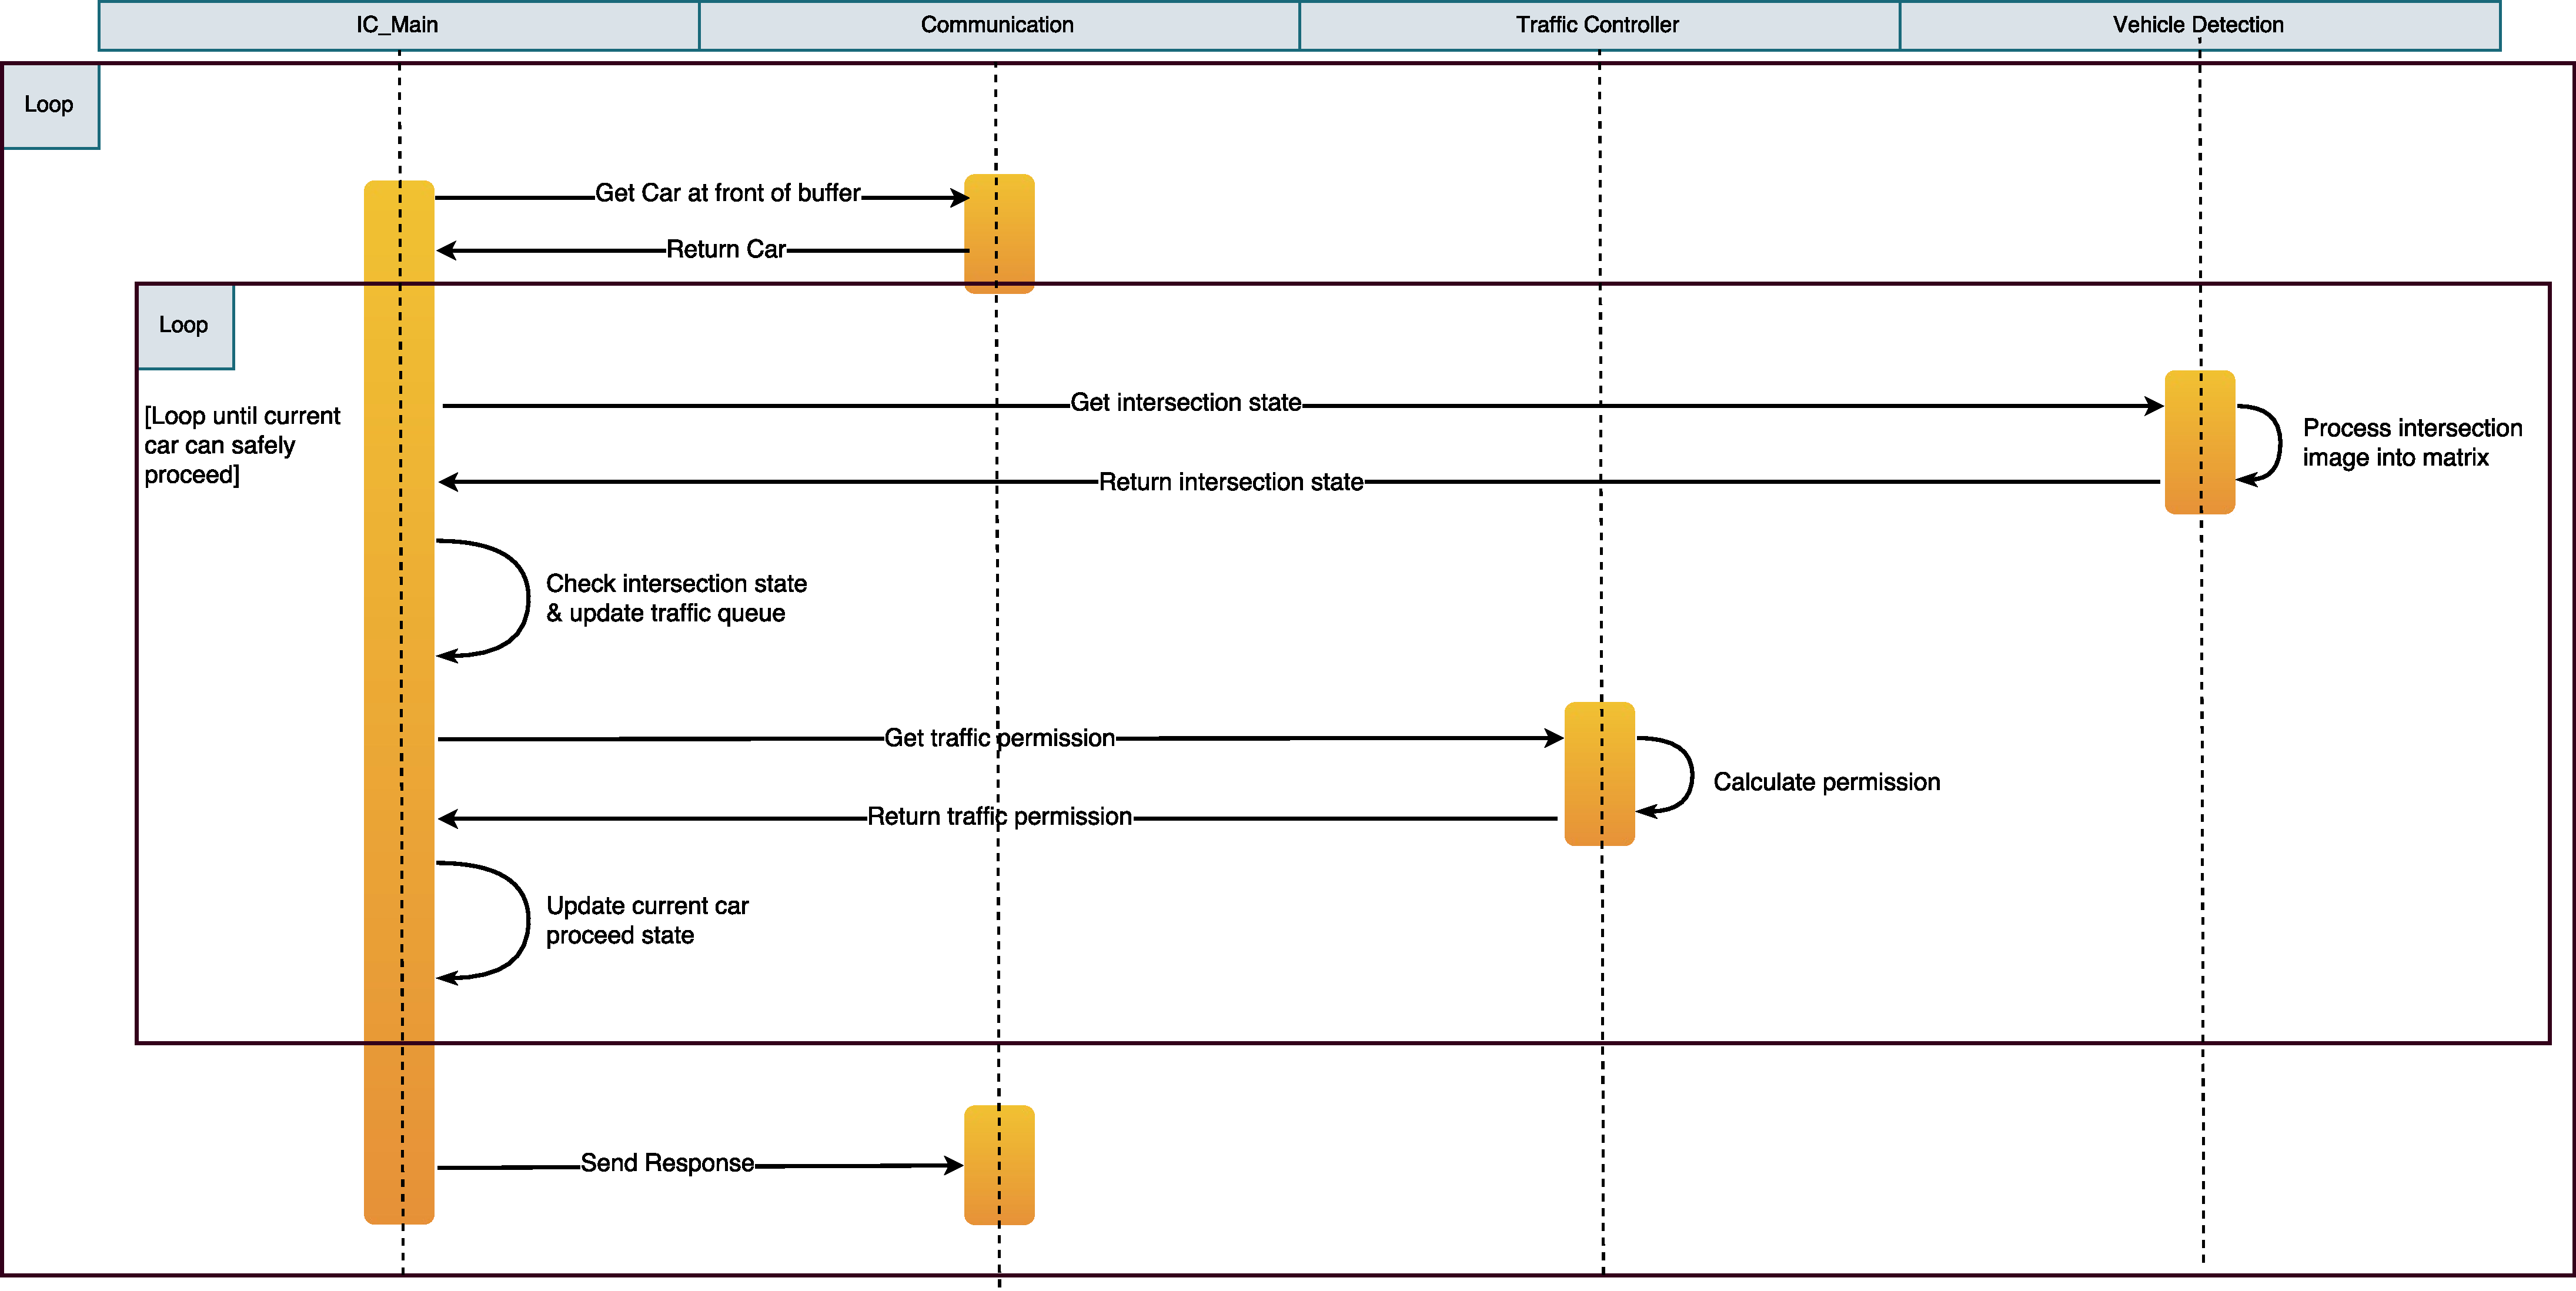
\includegraphics [scale = .3, angle = 90, trim={0 0 0 0},clip] {figures/IC_Sequence_Diagram.pdf}

\end {figure}


\begin {figure}[h!]
\centering
\caption{Intersection Component Sequence Diagram} \vspace{4mm}
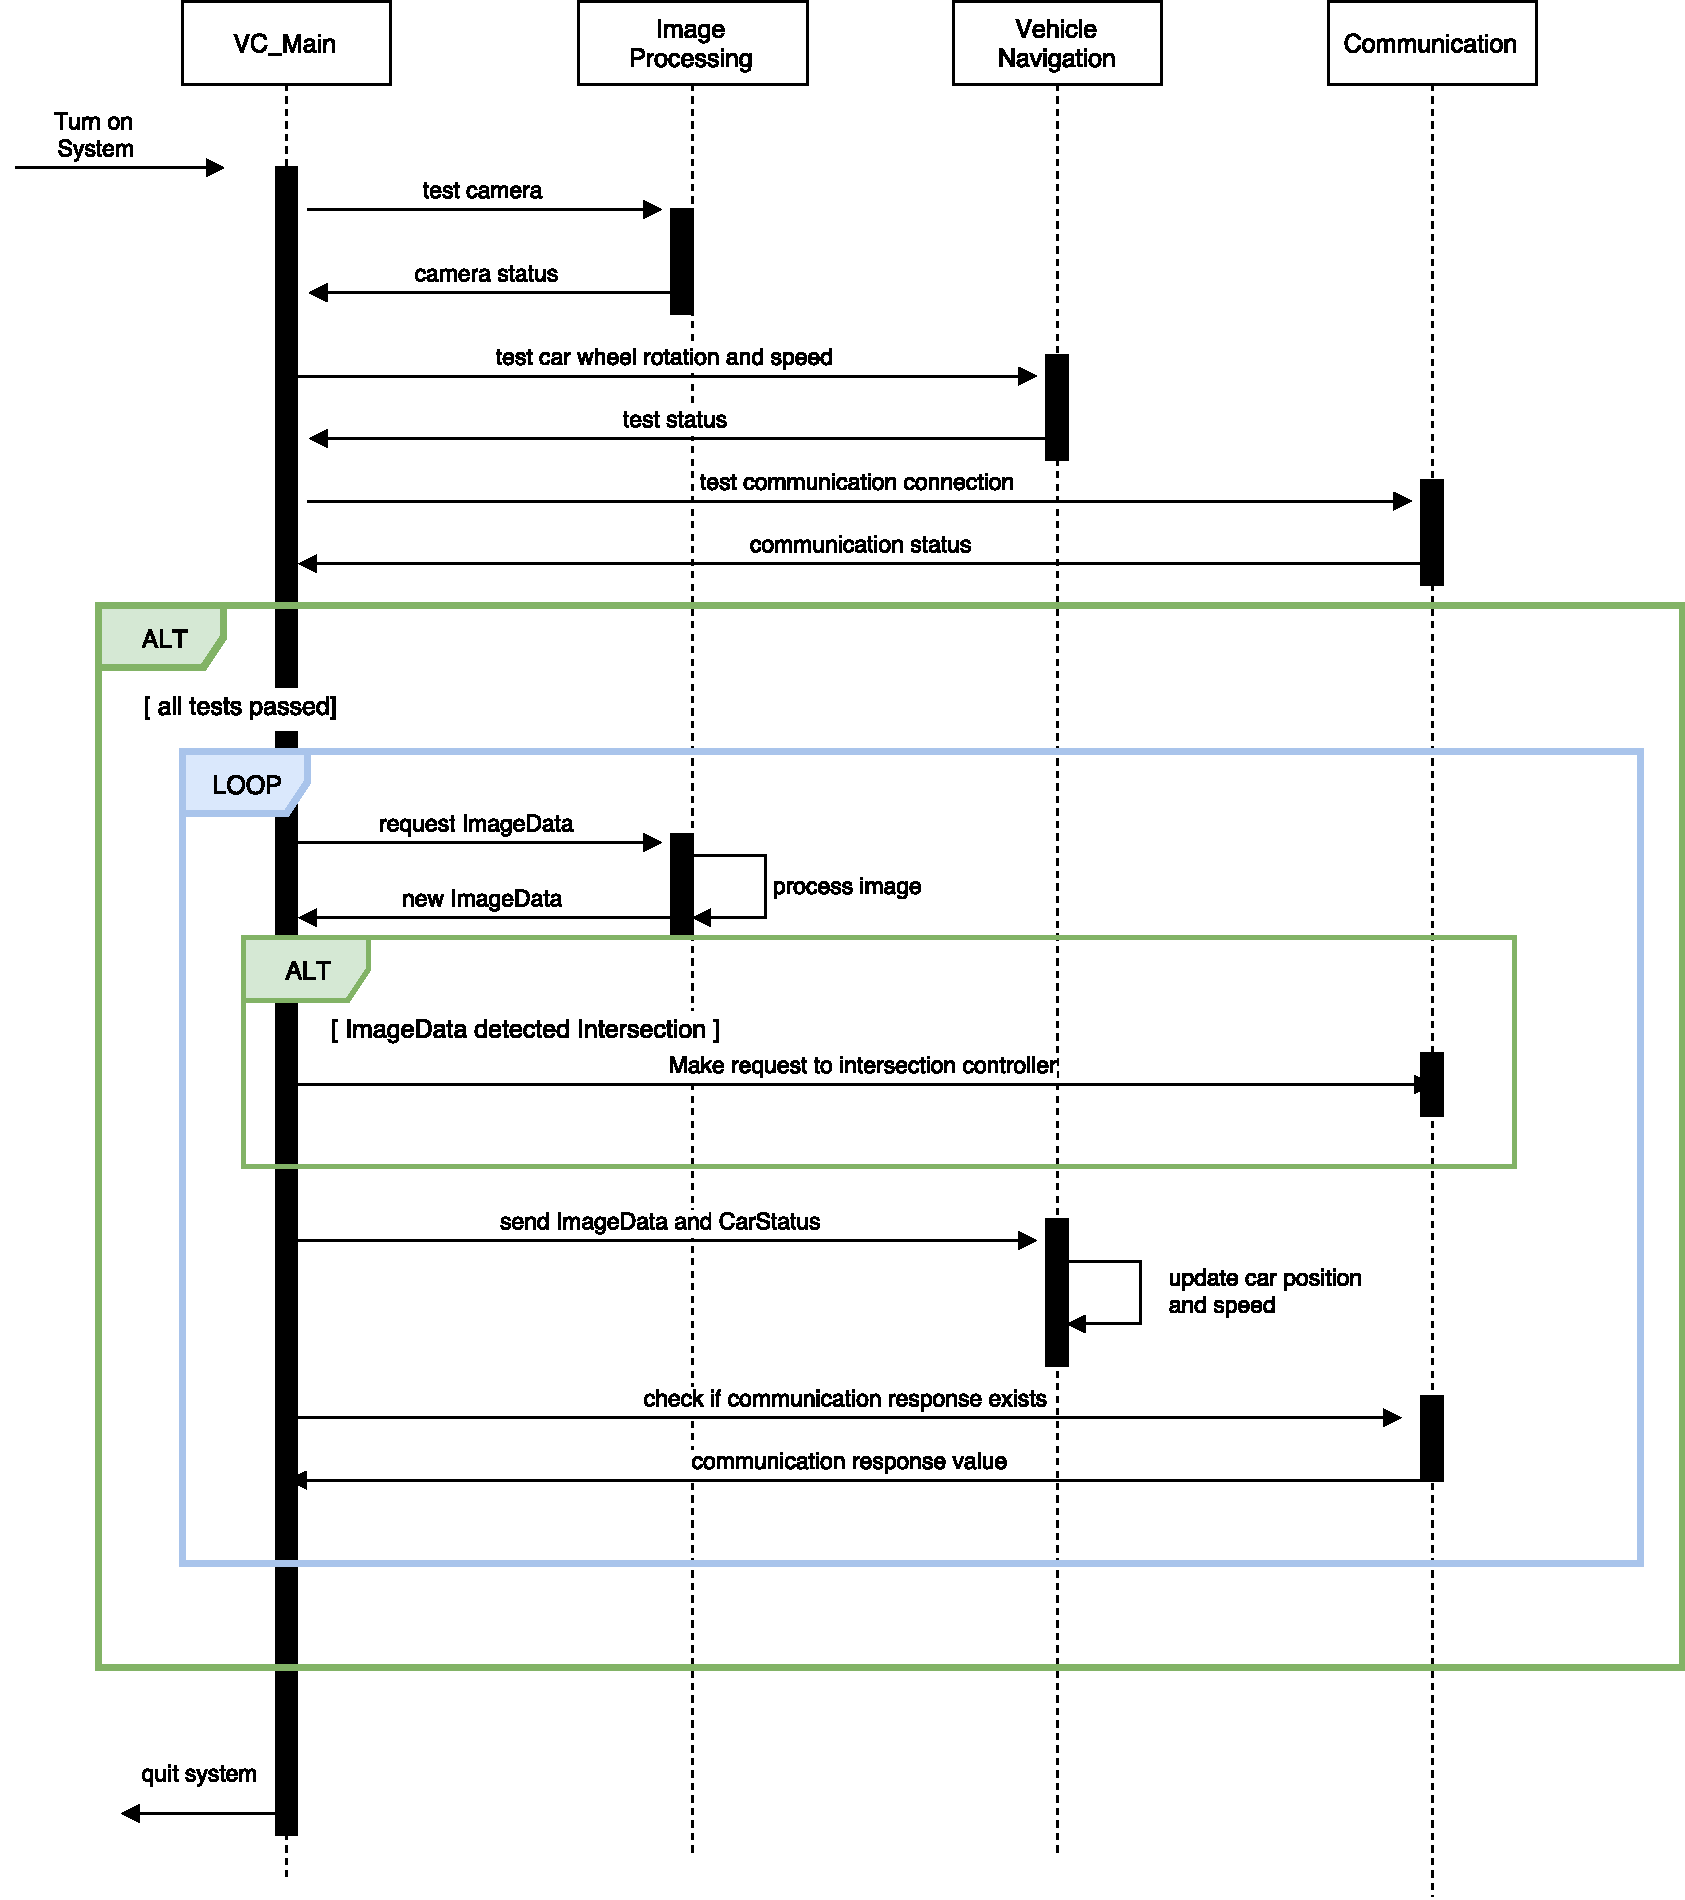
\includegraphics [scale = .6, trim={0 0 0 0},clip] {figures/carSequenceDiag.pdf}

\end {figure}


%\section{Design Notes}
%Insert Text Here.

% \section{Data Dictionary (if necessary)}
% Insert Text Here.


% \section{References}
% Insert Text Here.


\end{document}
